\documentclass[conference]{IEEEtran}

%%% Packages
% \usepackage{array}
% \usepackage{amsmath}
% \usepackage{fancyhdr}
% \usepackage{graphicx}
% \usepackage{float}
% \usepackage[LGRgreek]{mathastext}
% \usepackage{lipsum}
% \usepackage{multirow}
% \usepackage{subfigure}
% \usepackage{url}
% \usepackage{varwidth,xcolor}
% \usepackage{tikz,xifthen}
% \usepackage{tikz-qtree}
% \usetikzlibrary{decorations.pathmorphing}
% \usetikzlibrary{fit}
% \usetikzlibrary{backgrounds}
% \usetikzlibrary{shapes,arrows,shadows}
% \usetikzlibrary{calc,decorations.pathreplacing,decorations.markings,positioning}
% \usetikzlibrary{snakes,decorations.text,shapes,patterns}

\usepackage[table]{xcolor}
%% The amssymb package provides various useful mathematical symbols
\usepackage{amssymb}

%% The amsthm package provides extended theorem environments
\usepackage{amsthm}

%% amsmath for math environment
\usepackage{amsmath}

\DeclareMathOperator*{\argmin}{arg\,min}
\DeclareMathOperator*{\argmax}{arg\,max}
\DeclareMathOperator*{\sign}{sign}
\DeclareMathOperator*{\infspie}{inf}


% to break equation
%\usepackage{mathpazo}
%\usepackage{mathptmx}
%\usepackage[mathpazo]{flexisym}
%\usepackage{breqn}

%% For clever reference
%\usepackage{cleveref}

%% color package
\usepackage{color}

%% figure package
\usepackage{epsf,graphicx}
\usepackage{epstopdf}
\usepackage{subfigure}
\usepackage{transparent}

%% New environment to have some indent inside enumerate environment
\usepackage{enumitem}

%% To create acronym for proper glossary
\usepackage{acro}

%% To number the line in the article
\usepackage{lineno}

%% Environment to include table with notes
\usepackage{array}
\usepackage{threeparttable}
\usepackage{booktabs}
\usepackage{multirow}
\usepackage{siunitx}

%% In order to change size of margin
\usepackage{geometry}
\usepackage{changepage}
\usepackage{lscape}
%% Colorpackage for table
\usepackage{colortbl}
\usepackage{tabularx}
\usepackage{arydshln}

%% To use URL referencing
\usepackage{url}
%\usepackage[hidelinks]{hyperref}

%% In order to draw some graphs
\usepackage{tikz,xifthen}
\usepackage{tikz-qtree}
\usetikzlibrary{decorations.pathmorphing} % noisy shapes
\usetikzlibrary{fit}					% fitting shapes to coordinates
\usetikzlibrary{backgrounds}	% drawing the background after the foreground
\usetikzlibrary{shapes,arrows,shadows}
\usetikzlibrary{calc,decorations.pathreplacing,decorations.markings,positioning}
\usetikzlibrary{snakes,decorations.text,shapes,patterns}
%\usepackage{scalefnt,lmodern,booktabs}

%% Paxkage for cross and tick symbols
\usepackage{pifont}
\newcommand{\cmark}{\color{green!60!black!80}\ding{51}}
\newcommand{\mmark}{{\color{green!60!black!80}\ding{51}}$^{!}$}
\newcommand{\xmark}{\color{red!60!black!80}\ding{55}}
\newcommand{\cmarksmall}{\color{green!60!black!80}\ding{51}}
\newcommand{\mmarksmall}{{\color{green!60!black!80}\ding{51}}$^{!}$}
\newcommand{\xmarksmall}{\color{red!60!black!80}\ding{55}}
\newcommand{\Conv}{\mathop{\scalebox{1.5}{\raisebox{-0.2ex}{$\ast$}}}}%

\definecolor{autoGuided}{rgb}{ 0.3765    0.7294    0.9412}
\newcommand{\autoGuidedColor}{(light-Blue)}
\definecolor{fullyAuto}{rgb}{ 0.0941    0.3843    0.6627}
\newcommand{\fullyAutoColor}{(dark-blue)}
\definecolor{semiAuto}{rgb}{ 0.0784    0.5059    0.1686}
\newcommand{\semiAutoColor}{(light-green)}
\definecolor{fullyGuided}{rgb}{ 0.4275    0.6902    0.3176}
\newcommand{\fullyGuidedColor}{(dark-green)}

\DeclareSIUnit\ppm{ppm}
\DeclareSIUnit\px{px}

\usepackage{ltxtable}
\usepackage{listings}
\usepackage{color}
%\usepackage[toc]{appendix}

\definecolor{codegreen}{rgb}{0,0.6,0}
\definecolor{codegray}{rgb}{0.5,0.5,0.5}
\definecolor{codepurple}{rgb}{0.58,0,0.82}
\definecolor{backcolour}{rgb}{0.95,0.95,0.92}

\lstdefinestyle{mystyle}{
    backgroundcolor=\color{backcolour},
    commentstyle=\color{codegreen},
    keywordstyle=\color{magenta},
    numberstyle=\tiny\color{codegray},
    stringstyle=\color{codepurple},
    basicstyle=\footnotesize,
    breakatwhitespace=false,
    breaklines=true,
    captionpos=b,
    keepspaces=true,
    numbers=left,
    numbersep=5pt,
    showspaces=false,
    showstringspaces=false,
    showtabs=false,
    tabsize=2
}

\lstset{style=mystyle}
\usepackage{setspace}


% Include acroyms
\usepackage{acro}
%\acrodef{cap}[CaP]{prostate cancer}
\DeclareAcronym{cap}{
short = CaP,
long = prostate cancer
}
%\acrodef{cade}[CADe]{computer-aided detection}
\DeclareAcronym{cade}{
short = CADe,
long = computer-aided detection
}
%\acrodef{cadx}[CADx]{computer-aided diagnosis}
\DeclareAcronym{cadx}{
short = CADx,
long = computer-aided diagnosis
}
\DeclareAcronym{lm}{
short = LM, 
long = Leung-Malik set
}
%\acrodef{us}[US]{ultrasound}
\DeclareAcronym{us}{
short = UTS,
long = ultrasound
}
%\acrodef{ct}[CT]{computer tomography}
\DeclareAcronym{ct}{
short = CT,
long = computer tomography
}
%\acrodef{cad}[CAD]{computer-aided detection and diagnosis}
\DeclareAcronym{cad}{
short = CAD,
long = computer-aided detection and diagnosis
}
%\acrodef{mri}[MRI]{magnetic resonance imaging}
\DeclareAcronym{mri}{
short = MRI,
long = magnetic resonance imaging
}
%\acrodef{nmr}[NMR]{nuclear magnetic resonance}
\DeclareAcronym{nmr}{
short = NMR,
long = nuclear magnetic resonance
}

\DeclareAcronym{omp}{
  short = OMP,
  long =  orthogonal matching pursuit 
}
\DeclareAcronym{adb}{
  short = AdB, 
  long = AdaBoost
}
\DeclareAcronym{gb}{
  short = GB, 
  long = Gradient Boosting
}

\DeclareAcronym{mp}{
  short = MP,
  long =  Matching Pursuit 
}
%\acrodef{t2w}[T$_2$-W]{T$_2$ Weighted}
\DeclareAcronym{t2w}{
short = T$_2$-W,
long = T$_2$ Weighted
}
%\acrodef{dce}[DCE]{dynamic contrast-enhanced}
\DeclareAcronym{dce}{
short = DCE,
long = dynamic contrast-enhanced
}
%\acrodef{dw}[DW]{diffusion weighted}
\DeclareAcronym{dw}{
short = DW,
long = diffusion weighted
}
%\acrodef{mrsi}[MRSI]{magnetic resonance spectroscopy imaging}
\DeclareAcronym{mrsi}{
short = MRSI,
long = magnetic resonance spectroscopy imaging
}
%\acrodef{bph}[BPH]{benign prostatic hyperplasia}
\DeclareAcronym{bph}{
short = BPH,
long = benign prostatic hyperplasia
}
%\acrodef{pz}[PZ]{peripheral zone}
\DeclareAcronym{pz}{
short = PZ,
long = peripheral zone
}
%\acrodef{cz}[CZ]{central zone}

\DeclareAcronym{mpmri}{
short = mp-MRI,
long = multiparametric \ac{mri}
}
\DeclareAcronym{cz}{
short = CZ,
long = central zone
}
%\acrodef{tz}[TZ]{transitional zone}
\DeclareAcronym{tz}{
short = TZ,
long = transitional zone
}
%\acrodef{cg}[CG]{central gland}
\DeclareAcronym{cg}{
short = CG,
long = central gland
}
%\acrodef{psa}[PSA]{prostate-specific antigen}
\DeclareAcronym{psa}{
short = PSA,
long = prostate-specific antigen
}
%\acrodef{trus}[TRUS]{transrectal ultrasound}
\DeclareAcronym{trus}{
short = TRUS,
long = transrectal ultrasound
}
%\acrodef{tr}[TR]{repetition time}
\DeclareAcronym{tr}{
short = TR,
long = repetition time
}
%\acrodef{te}[TE]{echo time}
\DeclareAcronym{te}{
short = TE,
long = echo time
}
%\acrodef{si}[SI]{signal intensity}
\DeclareAcronym{si}{
short = SI,
long = signal intensity
}
%\acrodef{ees}[EES]{extravascular-extracellular space}
\DeclareAcronym{ees}{
short = EES,
long = extravascular-extracellular space
}
%\acrodef{t1w}[T$_1$-W]{T$_1$ Weighted}
\DeclareAcronym{t1w}{
short = T$_1$-W,
long = T$_1$ Weighted
}
%\acrodef{fse}[FSE]{Fast Spin-Echo}
\DeclareAcronym{fse}{
short = FSE,
long = Fast Spin-Echo
}
%\acrodef{adc}[ADC]{Apparent Diffusion Coeffient}
\DeclareAcronym{adc}{
short = ADC,
long = apparent diffusion coefficient
}
%\acrodef{roi}[ROI]{region of interest}
\DeclareAcronym{roi}{
short = ROI,
long = region of interest
}
%\acrodef{cse}[CSE]{chemical shift effect}
\DeclareAcronym{cse}{
short = CSE,
long = chemical shift effect
}
%\acrodef{snr}[SNR]{signal-to-noise}
\DeclareAcronym{snr}{
short = SNR,
long = signal-to-noise
}
\DeclareAcronym{se}{
short = SE, 
long = sensitivity
}
\DeclareAcronym{sp}{
short = SP, 
long = specificity
}
%\acrodef{gs}[GS]{Gleason score}
\DeclareAcronym{gs}{
short = GS,
long = Gleason score
}
%\acrodef{ersspc}[ERSSPC]{European Randomized Study of Screening for Prostate Cancer}
\DeclareAcronym{ersspc}{
short = ERSSPC,
long = European randomized study of screening for prostate cancer
}
%\acrodef{plco}[PLCO]{Prostate, Lung, Colorectal and Ovarian}
\DeclareAcronym{plco}{
short = PLCO,
long = prostate lung colorectal and ovarian
}
%\acrodef{fig}[Fig.]{figure}
\DeclareAcronym{fig}{
short = Fig.,
long = figure,
class = latex
}
\DeclareAcronym{tab}{
short = Table,
long = table,
class = latex
}
\DeclareAcronym{eq}{
short = Eq.,
long = equation,
class = latex
}
\DeclareAcronym{sec}{
short = Sect.,
long = section,
class = latex
}
\DeclareAcronym{chp}{
short = Chap.,
long = Chapter,
class = latex
}

\DeclareAcronym{fov}{
short = FOV,
long = field of view
}
\DeclareAcronym{dwt}{
short = DWT,
long = discrete wavelet transform
}
\DeclareAcronym{dwst}{
short = DWST,
long = discrete wavelet squared transform
}
\DeclareAcronym{map}{
short = MAP,
long = maximum \textit{a posteriori}
}
\DeclareAcronym{ml}{
short = ML,
long = maximum likelihood
}
\DeclareAcronym{mle}{
short = MLE,
long = maximum likelihood estimation
}
\DeclareAcronym{mrf}{
short = MRF,
long = Markov random field
}
\DeclareAcronym{itk}{
short = ITK,
long = Insight Segmentation and Registration Toolkit
}
\DeclareAcronym{es}{
short = ES,
long = Evolution Strategy
}
\DeclareAcronym{scf}{
short = SCF,
long = sparse coded features
}
\DeclareAcronym{bow}{
short = BoW,
long = bag of words
}
\DeclareAcronym{pdf}{
short = PDF,
long = probability density function
}
\DeclareAcronym{gscale}{
short = \textit{g}-scale,
long = generalized scale
}
\DeclareAcronym{aif}{
short = AIF,
long = arterial input function
}
\DeclareAcronym{svd}{
short = SVD,
long = singular value decomposition
}
\DeclareAcronym{mse}{
short = MSE,
long = mean squared error
}
\DeclareAcronym{mi}{
short = MI,
long = mutual information
}
\DeclareAcronym{mantra}{
short = MANTRA,
long = multi-attribute non-initializing texture reconstruction based active shape model
}
\DeclareAcronym{asm}{
short = ASM,
long = active shape model
}
\DeclareAcronym{pca}{
short = PCA,
long = principal components analysis
}
\DeclareAcronym{weritas}{
short = WERITAS,
long = weighted ensemble of regional image textures for active shape model segmentation
}
\DeclareAcronym{staple}{
short = STAPLE,
long = simultaneous truth and performance level estimation
}
\DeclareAcronym{lda}{
short = LDA,
long = linear discriminant analysis
}
\DeclareAcronym{lbp}{
short = LBP,
long = local binary pattern
}
\DeclareAcronym{tps}{
short = TPS,
long = thin plate spline
}
\DeclareAcronym{acm}{
short = ACM,
long = active contour model
}
\DeclareAcronym{cmi}{
short = CMI,
long = combined mutual information
}
\DeclareAcronym{svm}{
short = SVM,
long = support vector machines
}
\DeclareAcronym{rvm}{
short = RVM,
long = relevant vector machine
}
\DeclareAcronym{rbf}{
short = RBF,
long = radial basis function
}
\DeclareAcronym{knn}{
short = $k$-NN,
long = $k$-nearest neighbour
}
\DeclareAcronym{nn}{
short = NN,
long = neareast neighbour
}
\DeclareAcronym{dct}{
short = DCT,
long = discrete cosine transform
}
\DeclareAcronym{hog}{
short = HOG,
long = histogram of oriented gradient
}
\DeclareAcronym{dft}{
short = DFT,
long = discrete fourier transform
}
\DeclareAcronym{us1}{
short = US,
long = under-sampling
}
\DeclareAcronym{os}{
short = OS,
long = over-sampling
}
\DeclareAcronym{ros}{
short = ROS,
long = random-over-sampling
}
\DeclareAcronym{rus}{
short = RUS,
long = random-under-sampling
}
\DeclareAcronym{nm}{
short = NM,
long = nearmiss
}
\DeclareAcronym{nm3}{
short = NM-3,
long = nearmiss-3
}
\DeclareAcronym{nm2}{
short = NM-2,
long = nearmiss-2
}
\DeclareAcronym{nm1}{
short = NM-1,
long = nearmiss-1
}
\DeclareAcronym{iht}{
short = IHT,
long = instance-hardness-threshold
}
\DeclareAcronym{smote}{
short = SMOTE,
long = synthetic minority over-sampling techniques
}
\DeclareAcronym{smoteb1}{
short = SMOTE-b1,
long = SMOTE-borderline1
}
\DeclareAcronym{smoteb2}{
short = SMOTE-b2,
long = SMOTE-borderline2
}
\DeclareAcronym{mrmr}{
short = mRMR,
long = minimum redundancy maximum relevance
}
\DeclareAcronym{lle}{
short = LLE,
long = locally linear embedding
}
\DeclareAcronym{ica}{
short = ICA,
long = independent components analysis
}
\DeclareAcronym{qda}{
short = QDA,
long = quadratic discriminant analysis
}
\DeclareAcronym{id3}{
short = ID3,
long = iterative dichotomiser 3
}
\DeclareAcronym{cart}{
short = CART,
long = classification and regression tree
}
\DeclareAcronym{bagging}{
short = bagging,
long = bootsrap aggregating
}
\DeclareAcronym{loo}{
short = LOOCV,
long = leave-one-out cross-validation
}
\DeclareAcronym{lopo}{
short = LOPO CV,
long = leave-one-patient-out cross-validation
}

\DeclareAcronym{kcv}{
short = $k$-CV,
long = $k$-fold cross-validation
}
\DeclareAcronym{roc}{
short = ROC,
long = receiver operating characteristic
}
\DeclareAcronym{froc}{
short = FROC,
long = free-response receiver operating characteristic
}
\DeclareAcronym{auc}{
short = AUC,
long = area under the curve
}
\DeclareAcronym{rmse}{
short = RMSD,
long = root-mean-square deviation
}
\DeclareAcronym{rms}{
  short = RMS,
  long = root mean square
}
\DeclareAcronym{srsf}{
  short = SRSF,
  long =  square-root slope function
}
\DeclareAcronym{pun}{
short = PUN,
long = phenomenological universalities
}
\DeclareAcronym{etl}{
short = ETL,
long = echo train ength
}

\DeclareAcronym{rf}{
short = RF,
long = random forest
}
\DeclareAcronym{dna}{
short = DNA,
long = deoxyribonucleic acid
}

\DeclareAcronym{glcm}{
short = GLCM,
long = gray-level co-occurence matrix
}

\DeclareAcronym{iccvb}{
short = I2Cvb,
long = initiative for collaborative computer vision benchmarking
}

\DeclareAcronym{mloss}{
short = MLOSS 2015,
long = machine learning open source software 2015
}

\DeclareAcronym{ci}{
short = CI,
long = continuous integration
}

\DeclareAcronym{cern}{
short = CERN,
long = european organization for nuclear research
}

\DeclareAcronym{doi}{
short = DOI,
long = digital object identifier
}

\DeclareAcronym{pd}{
short = PD,
long = proton density
}

\DeclareAcronym{anova}{
short = ANOVA,
long = analysis of variance
}


%%% Document
\begin{document}

%%Command to thanks
% \IEEEoverridecommandlockouts

%% Command to meet the printer requirements
%\overrideIEEEmargins

% Authors
% Author(s) Name(s)
\def \AuthorA{Guillaume Lema\^{i}tre}
\def \AuthorB{Robert Mart\'i}
\def \AuthorC{Mojdeh Rastgoo}
\def \AuthorD{Fabrice M\'eriaudeau}

% Author(s) Email(s)
\def \AuthorAemail{fabrice.meriaudeau@utp.edu.my}

% Institution(s) Name(s)
\def \InstitutionA{\small Parietal team, Inria, CEA, Universit\'e Paris-Saclay,
1 Rue Honor\'e d'Estienne d'Orves, 91120 Palaiseau}
\def \InstitutionB{\small LE2I UMR6306, CNRS, Arts et M\'etiers,
  Univ. Bourgogne Franche-Comt\'e, 12 rue de la Fonderie, 71200 Le
  Creusot}
\def \InstitutionC{\small ViCOROB, Universitat de Girona, Campus Montilivi,
  Edifici P4, 17071 Girona}
\def \InstitutionD{\small CISIR, Electrical \& Electronic Engineering Department,
  Universiti Teknologi Petronas, 32610 Seri Iskandar, Perak}

% Article title
\title{\LARGE \bf
 Computer-Aided Detection for Prostate Cancer Detection based on
 Multi-Parametric Magnetic Resonance Imaging}

\author{\AuthorA\authorrefmark{1}, \AuthorB\authorrefmark{2},
  \AuthorC\authorrefmark{3}, \AuthorD\authorrefmark{4}\authorrefmark{5}\\
\authorblockA{\authorrefmark{1}\InstitutionA}
\authorblockA{\authorrefmark{2}\InstitutionC}
\authorblockA{\authorrefmark{3}\InstitutionB}
\authorblockA{\authorrefmark{4}\InstitutionD}
\authorblockA{\authorrefmark{5}\small Corresponding author: \AuthorAemail}
}

%%% Local Variables:
%%% mode: latex
%%% TeX-master: "main"
%%% End:


\maketitle
%\thispagestyle{plain}
%\pagestyle{plain}

% Abstract
\begin{abstract}
\Ac{cap} is the second most diagnosed cancer in men all over the world.
In the last decades, new imaging techniques based on \ac{mri} have been developed improving diagnosis.
In practice, diagnosis is affected by multiple factors such as observer variability and visibility and complexity of the lesions.
In this regard, \ac{cad} systems are being designed to help radiologists in their clinical practice.
We propose a \ac{cad} system taking advantage of all MRI modalities (i.e., \acs*{t2w}-\acs*{mri}, \acs*{dce}-\acs*{mri}, \ac{dw}-\acs*{mri}, \acs*{mrsi}).
This system has been extensively tested on a dataset which has been made publicly available.
\end{abstract}

% Key words
\begin{IEEEkeywords}
Computer-Aided Diagnosis, Prostate Cancer, Normalization, Multi-Parametric MRI
\end{IEEEkeywords}
\IEEEpeerreviewmaketitle
\acresetall
% Sections
\section{Introduction}
Current \ac{cap} screening consists of 3 different stages.
First, \ac{psa} control is performed to distinguish between low- and
high-risk \ac{cap}.
To assert such diagnosis, samples are taken during prostate biopsy and
analyzed to make an accurate prognosis of the \ac{cap}.

Although \ac{psa} screening has been shown to improve early detection
of \ac{cap}~\cite{Chou2011}, its lack of reliability motivates further
investigations using \ac{mri}-based \ac{cad}.
Consequently, current research is focused on identifying new
biological markers to replace \ac{psa}-based
screening~\cite{Brenner2013}.
Until such research comes to fruition, these needs can be met through
active-surveillance strategy using \ac{mpmri}
techniques~\cite{Moore2013}.

%A general \ac{cad} work-flow is presented in \acs{fig}\,\ref{fig:wkfcad}.
%The \ac{cad} work-flow is presented in \acs{fig}~\ref{fig:wkfcad}.
Lemaitre\,\emph{et~al.} recently reviewed
more than 50 research works that focused on \ac{cad} system for
\ac{cap}~\cite{Lemaitre2015}.
These studies are based on \ac{cad} systems that consists of the
following steps:
(i) pre-processing,
(ii) segmentation,
(iii) registration,
(iv) feature detection,
%(v) feature balancing,
(v) feature selection-extraction, and
(vi) finally classification.

The reviewed \ac{mpmri}-based \ac{cad} used 2 to 3
\ac{mri} modalities among \ac{t2w}-\ac{mri}, \ac{dce}-\ac{mri}, and
\ac{dw}-\ac{mri}, discarding the potential discriminative power of
\ac{mrsi}.
Furthermore, only half of these studies tackled the challenging
detection of \ac{cap} in the \ac{cg}.
Additionally, none of the works investigated the issue related to
feature balancing when developing their \ac{cad} systems.
Finally, none of the datasets nor source codes used have been
released, making impossible the possibilities to compare the methods.

%In \iac{cade} framework, \textit{possible lesions are segmented
%automatically} and further used as input of \iac{cadx}.
%Nevertheless, some works also used a fusion of \ac{cade}-\ac{cadx}
%framework in which a voxel-based features are directly used, in which
%the location of the malignant lesions are obtained as results.
%On the other hand, manual lesions segmentation is not considered to
%be part of \ac{cade}.
%The output of the \ac{cade} is used as input of the \ac{cadx}.

%$\Ac{cadx} is composed of the processes allowing to
%\textit{distinguish malignant from non-malignant tumours}.
%Here, \ac{cap} malignancy is defined using the grade of the \ac{gs}
%determined after post biopsy or prostatectomy.
%As presented in \ac{fig}\,\ref{fig:wkfcad}, \ac{cadx} is usually
%composed of the three common steps used in a classification
%framework: (i) features detection, (ii) feature extraction/selection,
%and (iii) feature classification.

In this work, we propose a \ac{cad} system to detect \ac{cap} in
\ac{pz} and \ac{cg}, using the 4 aformentioned \ac{mri}
modalities.
In addition, our framework include a step of feature balancing.
The dataset used and the source code developed are released for future
comparisons and reproducibility.

% \section{Denoising Algorithms} \label{sc:methodology}
%%We can add kind of intro to this section


%\subsection{Traditionnal filters}

In this paper, a set of conventional filters are used: (i) a mean filter, (ii) a median filter, (iii) a local statistics filter (i.e. Lee filter~\cite{4766994}), (iv) hard and soft thresholding in wavelet domain~\cite{wavelet}, and (v) \ac{nlm}~\cite{nlm}. The more recent techniques used are described below.

%Filter Given a noisy image $g$, the restored value on the denoised image $\hat{f}$ at the position $(x, y)$ corresponds to the average of the neighbourhood $N$ (See Eq. \ref{eq:mean-filter}).

%\begin{equation}
	%\hat{f}(x, y) = \frac{1}{M\cdot N}\sum_{(u, v) \in N(x, y)}{g(x, y)}.
    %\label{eq:mean-filter}
%\end{equation}

%This process acts on the supposition that the noise is concentrated on the upper part of the frequency spectrum. This approach is able to remove pixels which are not representative in the considered neighborhood and also reduce the noise by blurring the image. Thus, high frequencies are lost during the process.

%This is the simplest denoising technique and it is not  very effective (but was tested as a comparison). Denoising through a mean filter simply applies a linear transformation of the input image  (a convolution with a smoothing kernel), and it makes no attempt to interpret the information in the image and use it in the denoising process.


%\subsection{Median filter}

%Median filter is a spatial filter based on order-statistics. It replaces the intensity value at each position with the 50th percentile of the neighborhood (See Eq. \ref{eq:median-filter}). 

%\begin{equation}
	%\hat{f}(x, y) = {median}_{\substack{(u, v) \in N(x, y)}}{g(x, y)}.
    %\label{eq:median-filter}
%\end{equation}

%Unlike mean filter, median filter is able to detect outliers of a neighborhood and remove them with a smaller impact on the higher frequencies. For the same reason, this filter is providing good results onto  images affected by salt-and-pepper noise. 

%The main drawback of this method is its computational complexity for large groups of data. % What? No!

%subsection{Filtering by use of local statistics (LS filter)}
%Digital Image enhancement by using local statistics is a computational technique that involves contrast and noise filtering on two-dimensional arrays based on their local mean and variance. One of the greatest advantages of this type of algorithms is that they are non-recursive and each pixel is processed independently. As a consequence this approach has a great advantage when  used in real time image processing.
%The assumption of the algorithm based on local statistics is that the sample mean and variance of a pixel is equal to the local mean and variance of all the pixels within a fixed range.

%This simple approach has been pointed as to lack mathematical elegance and sophistication, compared to other techniques, however the results indicate it is a very effective tool for contrast stretching and noise filtering of images.

%et $x_{ij}$ be the brightness of the pixel $(i,j)$ in a two dimensional $N\times N$ image. The local mean and variance are then calculated over a $(2n+1) \times (2m+1)$ window. The local mean is defined as:

%\begin{equation}
    %\mu_{ij}=\dfrac{1}{(2n+1)(2m+1)}\sum_{k=i-n}^{n+i}\sum_{l=j-m}^{m+j}{x_{kl}},
    %\label{eq:ls_filter_1}
%\end{equation}

%and the local variance is:

%\begin{equation}
   % v_{j} =\dfrac{1}{(2n+1)(2m+1)} \sum_{k=i-n}^{i+m}\sum_{l=j-m}^{j+m} (x_{kl} - \mu_{ij} )^2.
    %\label{eq:ls_filter_2}
%\end{equation}

%From these equations it is not hard to extend the algorithm to deal with images corrupted by additive or multiplicative noise or even both. A noisy corrupted image is described as: 

%\begin{equation}
%z_{ij} = x_{ij}*u_{ij} + w_{ij}.
    %\label{eq:ls_filter_3}
%\end{equation}

%Where the mean and variance are calculated as:

%\begin{equation}
    %E[(u_{ij} - \vec{u_{ij}})( u_{kl} -\vec{u_{kl}})] = \sigma^2*\delta_{ik}*\delta_{jl}.
    %\label{eq:ls_filter_4}
%\end{equation}

%From the structure of the algorithm, it is easy to see that the principal computational load relays on the calculation of the local mean and variance of the image. To make the calculations faster, an improvement to the algorithm is proposed where the image is partitioned in square sub regions over which the local variance and mean are calculated. Further, the local mean and variance of a pixel are approximated by the use of two dimensional interpolation formulas. This improvement seems to be promising and perfectly suitable for real time -parallel image processing.

%\subsection{Hard and soft thresholding in wavelet domain (wavelet filter)}


%The wavelet transform is used extensively in signal de-noising. The usual way to de-noise signals in wavelet domain is to first transform the signal into wavelet domain, apply hard or soft thresholding and then transform back. 

%Hard thresholding is a noise suppression method, that applies the following transformation to the empirical wavelet coefficients:

%\begin{equation}
   % F(x)=x\cdot I(|x|>t),
   %\label{eq:wavelet_1}
%\end{equation}

%where $t$ is a threshold value. For de-noising to perform adequately, $t$ must be chosen carefully.

%The theoretically optimal value for $t$ is $t=\sqrt{2\sigma^{2}log(n)/n}$, where $\sigma^{2}$is the variance of the noise and $n$ is the length of input data. In practice, usually, a smaller value is usually used ~\cite{thresholding}.

%Soft thresholding, just like hard thresholding, incorporates a transformation of the empirical wavelet coefficients. The only difference is the chosen nonlinear transformation:

%\begin{equation}
    %S(x)=sign(x)(|x|-t)\cdot I(|x|>t),
    %\label{eq:wavelet_2}
%\end{equation}

%where, again, $t$ is the threshold value.

%However, when the signal contains discontinuities, the denoising will also result in artifacts: pseudo-Gibbs phenomena, when the signal is alternatively overshooting or undershooting its level. These artifacts depend on the precise alignment between the signal and the basis elements, therefore depend both on wavelets and the input data. 

%A solution was proposed in "Translation-Invariant De-Noising"~\cite{wavelet}, where Coifman and Donoho present an algorithm to minimize the effects of this phenomenon. 



\subsection{\acf{ssdc} approach}
This technique is based on the paper of Yahya~\emph{et~al.}~\cite{6717020}; first, the speckle noise is converted from multiplicative to additive via homomorphic filtering and later the vector space of the noisy image is decomposed into signal and noise subspaces.
The enhancement occurs by canceling the noise subspsace and estimating through a linear estimator the clean image from the remaining signal subspace. 

\subsection{\acf{bm3d}}
\ac{bm3d} is an image denoising strategy which uses block matching and collaborative filtering in the 3D domain~\cite{dabov2007image}.
The core algorithm is composed of three steps: (i) grouping, (ii) collaborative filtering, and (iii) aggregation.
The first step consists in grouping similar 2D image patches from different spatial locations, to form 3D blocks.
The collaborative filtering is equivalent to denoise the 3D blocks by successively applying a 3D transform, a denoising method, and an inverse 3D transform.
Finally, a denoised image is reconstructed by making a linear combination of the 2D denoised patches.

The previous algorithm is applied twice in the \ac{bm3d} framework to build: (i) a basic estimate and (ii) a final estimate.
More precisely, the basic estimate is computed by grouping noisy 2D patches, denoising the blocks via hard-thresholding, and aggregating the patches by setting the weights to be inversely proportional to the total sample variance of the blocks.
Then, the grouping in the final estimate is built from two distinct blocks by arranging 2D patches from both the noisy image and basic estimate.
The filtering is performed through a Wiener filter driven by the blocks extracted from the basic estimate, considered as the true energy spectrum.
The aggregation step is equivalent to the one performed in the basic estimate stage to obtain the final denoised image.


%The aim of block matching is to stack similar 2D image fragments ("blocks"), in 3D arrays called "groups".
%Similarities are computed between candidate fragments at different spatial locations and each reference fragment.
%The groups are disjoints, so some blocks can be stacked in multiple groups.
%These groups have a "diameter" corresponding to the maximum number of blocks that they contained.

%After getting the groups by block matching, a collaborative filtering is applied, which include: 3D transformation, shrinkage of the transform spectrum, and inverse 3D transform.
%Different 3D transformations can be applied according to the type of noise, or it can be decomposed in 2D transform followed by 1D transform.

%The last process used is the aggregation.
%Because the groups are disjoints, multiple estimates are given for some blocks so that they will overlap.
%In order to aggregate them, the blocks are awarded with weights.
%For each final pixel, the block pixels correspond to the average with their given weights.

%The algorithm is divided in two steps.
%The first one consists in applying block matching and collaborative filtering on the noisy image.
%The shrinkage of the coefficients of the 3D group is realised for this first step with an hard-thresholding filter.
%The basic estimate got from the first step helps to improves an other block matching in the second step.
%Collaborative filtering is applied once again on these new obtained blocks and the shrinkage is now realised by a Wiener filter, which attenuates the frequencies using %the signal to noise ratio.
%The final estimate is therefore obtained, what corresponds to the denoised image.

%Multiple parameters can be tuned in order to choose between a faster or more accurate algorithm, such as: block size, group diameter, step between reference blocks, and search area.

%This method improves the \ac{nlm} filter method~\cite{nlm} in using 3D transform instead of 1D.
%Thanks to the filtering in transform domain applied on the already process groups, the method preserves uniform areas, smooth intensity transitions, textures, repeating patterns, and sharp edges.
%The main advantages of this approach is the non-locality and the collaborative filtering

\subsection{K-SVD} \label{sc:description-ksvd}
This denoising method consists in decomposing images using sparse and redundant representations over trained dictionaries.
The authors in~\cite{ksvd} propose two possible implementations: (i) with a pre-trained dictionary learnt from high quality natural images and using the \ac{dct}, or (ii) by training a new dictionary using the corrupted one.
We chose the first option with an overcomplete \ac{dct} dictionary since that this option leads to better performance.

%\subsection{NLM}

%Non local means (NL-means) algorithm for image denoising in ~\cite{nlm} is based on a non-local averaging of all pixels in the image. The main difference of the NL-means algorithm compared to local filters or frequency domain filters is the systematic use of all possible self-predictions the image can provide, a principle used also in ~\cite{texture}.  

%Non local means algorithm is based on the following equation:

%\begin{equation}
%	\begin{split}
%		NL&[u](x)=\\
 %       &\frac{1}{C(x)}\int_{\Omega} e^{-\frac{(G_a*\mid u(x+.)-u(y+.)\mid ^2(o))}{h^2}}u(y)dy,
%	\end{split}
%\end{equation}
%where $x \epsilon\, \in\,  \Omega$,
%\begin{equation}
%	\begin{split}
%	    C(x)&= \\
 %       &\int_{\Omega} e^{-\frac{(G_a*\mid u(x+.)-u(y+.)\mid ^2(o))}{h^2}}u(y)dy
  %  \end{split}
%\end{equation}
%is a normalizing constant, $h$ is the filtering parameter and $G_a$ is a Gaussian kernel. The new value of a pixel $x$ is defined as the mean of all the pixels in the image whose neighborhood is similar to the neighborhood of $x$.

%\begin{equation}
%	NL[v](i)=\sum_{j\space\epsilon\space I}{w(i,j)\cdot v(i,j)},
%\end{equation}

%where $v= \{v(i)  \mid  i \in I \}$ represents all the pixels in an Image and the weights for each pixel depend on the similarity between the two pixels I and j. The weights {w(i,j)}, depend on the similarity between two pixels I and j under the conditions: $0 < w(i,j)< 1,\,\sum_{j}{w(i,j)}=1$.

%The similarity between two pixels i,j is determined by the similarity of the intensity gray level vectors $v(N_i)$ \& $v(N_j)$ of square neighborhoods of fixed size. This similarity index is defined by the weighted Euclidean distance $\parallel v(N_i )-v(N_j ) \parallel _{(2,a)}^2$  where $a > 0$ is the Euclidean distance between the two noisy neighborhoods, making the system robust:

%\begin{equation}
%	E\parallel v(N_i )-v(N_j )\parallel_{(2,a)}^2=
 %   \parallel u(N_i )-u(N_j ) \parallel _{2,a}^2+2 \sigma^2.
%\end{equation}

%The weights are defined as 
%\begin{equation}
%w(i,j)=\frac{1}{Z(i)} e^\frac{-\parallel v(N_i)-u(N_j) \parallel _{2,a}^2 }{h^2},
%\end{equation}

%where $Z(i)$ is the normalizing constant 

%\begin{equation}
%Z(i)=\sum_{j}{e^{\frac{-\parallel v(N_i)-u(N_j) \parallel _{2,a}^2 }{h^2}}}.
%\end{equation}

%The advantage of NLM denoising is that it not only compares the gray level with a single pixel but with the geometrical configuration of the neighborhood. 

\subsection{\acf{obnlm} filtering}

This method dedicated to ultrasound images is a modified version of the \ac{nlm} technique~\cite{obnlm}, to cope with the features of the speckle noise.
The \ac{nlm} algorithm analyses the patterns around the pixels rather than comparing intensity values which may be highly corrupted by noise.
For each pixel, the patches from the whole image are compared to find restoration parameters.
The modified algorithm proposes a Bayesian formulation of the \ac{nlm} filter inspired by~\cite{bayesian} which optimises the computational cost of the original algorithm. 

\subsection{\acf{pgpd}}
\ac{pgpd} is a recent patch-based technique proposed by Xu~\emph{et~al.}~\cite{xu2015patch}.
This method relies on a two-stage framework: (i) a learning stage and (ii) a denoising stage.
In the learning stage, non-local self-similar patches are grouped together and later modelled using a \ac{gmm}.
Then, for each component of the \ac{gmm}, a sparse dictionary is learnt.
In the denoising stage, the most suitable Gaussian component is selected with its corresponding dictionary and later used to denoise the image through a simple weighted sparse coding model.
% \section{Experiments and results}\label{sec:chp6:exp-res}

In this section, different experiments are proposed to design and
investigate our \ac{mpmri} \ac{cad} for the detection of \ac{cap}.
First, the classification performance of each independent modality is
investigated in \acs{sec}\,\ref{subec:chp6:exp-res:Ex1}.
For each modality, the ``quantification'' approaches maximizing the
classification performance are selected.
Additionally, we focus on to directly combined \ac{mpmri} modalities,
which we referred to as ``coarse'' combination as presented in
\acs*{sec}\,\ref{subsec:chp6:exp-res:Ex2}.
Subsequently, \acs{sec}\,\ref{subsec:chp6:exp-res:Ex3} presents the
benefit of balancing the dataset on the learning stage and strategies
for feature selection and extraction, for each feature modality as
well as an aggregation of them.
Consequently, different combination classifier rules are studied using
the previous fine-tuned feature space in
\acs{sec}\,\ref{subsec:chp6:exp-res:Ex4}.
Finally, we conclude in \acs{sec}\,\ref{subsec:chp6:exp-res:Ex5} by
investigating the benefit of fusing the \ac{mrsi} information with the
other modality.

All these experiments are conducted on a subset of the public
\ac{mpmri} prostate presented in \acs{sec}\,\ref{sec:data3t}.
We used the \SI{3}{\tesla} dataset which is composed of a total of 19
patients of which 17 patients had biopsy proven \ac{cap} and 2
patients are ``healthy'' with negative biopsies.
In this study, our subset consists of 17 patients with \ac{cap}.

\begin{landscape}
\begin{figure}
  \hspace*{\fill}
  \subfigure[Performance of the quantitative methods on
  \acs*{dce}-\acs*{mri}.]{\label{fig:inddcemodel}\includegraphics[height=.4\textheight]{5_normalization/figures/DCE-normalization/normalized_methods_0.pdf}}
  \hfill
  \subfigure[Performance of enhanced \acs*{dce}-\acs*{mri}
  signal.]{\label{fig:inddcesignal}\includegraphics[height=.4\textheight]{5_normalization/figures/DCE-normalization/full_signal_0.pdf}}
  \hspace*{\fill} \\
  \hspace*{\fill}
  \subfigure[Performance of image-based features for
  \acs*{t2w}-\acs*{mri} and \acs*{adc}
  map.]{\label{fig:indadct2w}\includegraphics[height=.4\textheight]{6_pipeline/figures/exp-1/t2w_adc.pdf}}
  \hfill
  \subfigure[Performance of different approaches for the \acs*{mrsi}
  modality.]{\label{fig:indmrsi}\includegraphics[height=.4\textheight]{6_pipeline/figures/exp-1/mrsi_all.pdf}}
  \hspace*{\fill}
  \caption[Analysis of the classification performance for each
  individual \acs*{mri} modality.]{Analysis of the classification
    performance for each individual \acs*{mri} modality. Different
    models have been tested for \acs*{dce}-\acs*{mri} and \acs*{mrsi}
    modalities.}
  \label{fig:res-Ex1}
\end{figure}
\end{landscape}

\subsection{Assessment of classification performance of individual modality}\label{subec:chp6:exp-res:Ex1}

In this experiment, we attend to assess the classification performance of each individual \ac{mri} modality.

\paragraph{\ac{t2w}-\ac{mri} and \ac{adc} map features} All features presented in \acs{tab}~\ref{tab:featureadct2w} are extracted for both \ac{t2w}-\ac{mri} and \ac{adc} map.
These features are combined per modality and for each of them, a \ac{rf} classifier is trained.

\paragraph{\ac{dce}-\ac{mri} features} This experiment has been presented in \acs{sec}\,\ref{subsec:chp5:DCE-norm:exp-res}.
We aim at finding the most discriminative ``quantification'' method for \ac{dce}-\ac{mri} modality, by assessing the classification performance of the different models.
Therefore, the pharmacokinetic parameters from the Brix, Hoffmann, Tofts, and \ac{pun} models, the semi-quantitative parameters, and the enhanced \ac{dce}-\ac{mri} signal are extracted.
For each set of feature, a \ac{rf} classifier is trained.

\paragraph{\ac{mrsi} features} Similarly to \ac{dce}-\ac{mri}, 4 \ac{rf} classifiers are trained on different features:
(i) the cropped \ac{mrsi} signal,
(ii) the relative concentration of the citrate over the relative concentration of the choline, both computed through fitting as presented in the previous section,
(iii) the ratio of the two previous features, and finally
(iv) the ratio of the relative concentration of the citrate over the relative concentration of the choline, using fix integration bounds.

\paragraph{Results}
Each trained \ac{rf} is evaluated using a \ac{lopo}.
A \ac{roc} analysis is carried out and the \ac{auc} score is computed to report and compare the classification performance of each classifier.
The results are depicted in \acs{fig}\,\ref{fig:res-Ex1}.
As presented is the previous chapter, classification of \ac{dce}-\ac{mri} data using the normalized enhanced \ac{dce}-\ac{mri} signal is the strategy leading the highest \ac{auc} --- i.e., $0.666 \pm 0.154$ ---, outperforming any quantification method.
Similarly to these findings, classification of the cropped \ac{mrsi} signal outperforms other quantification-based methods, with an \ac{auc} of $0.697 \pm 0.165$.
Classification of the extracted features based on \ac{adc} offer a close performance with an identical mean \ac{auc} and a smaller standard deviation of $0.128$.
Finally, the features extracted from \ac{t2w}-\ac{mri} are shown to be the most discriminative with an \ac{auc} reaching $0.720 \pm 0.122$.
As a conclusion, the most efficient features in terms of classification performance for each modality are selected for the remainder of the experiment section.

\subsection{Coarse combination of \acs*{mpmri} modalities} \label{subsec:chp6:exp-res:Ex2}

\begin{figure}
  \centering
  \includegraphics[width=0.7\linewidth]{6_pipeline/figures/exp-2/comb_all.pdf}
  \caption[Comparison of different combination approaches.]{Comparison of different combination approaches: (i) aggregation of the different features in conjunction with a \acs*{rf} classifier, (ii) a stacking approach using 4 \acs*{rf}s and \acs*{adb} as meta-classifier, and (iii) a stacking approach using 4 \acs*{rf}s and \acs*{gb} as meta-classifier.}
  \label{fig:res-Exp2}
\end{figure}

As a first attempt to design a \ac{mpmri} \ac{cad} system, 3 different approaches are used to combine the selected feature from each modality:
(i) feature aggregation,
(ii) stacking using \ac{adb},
(iii) stacking using \ac{gb}.
We refer these combinations as being coarse since no tuning --- i.e., feature balancing/selection/extraction --- aiming at improving the classification performance is involved.
This experiment can be considered as the baseline to obtain a \ac{mpmri} \ac{cad} for the detection of \ac{cap}.

In the first approach, the features from all the different modalities are concatenated together to form a unique matrix.
Additionally, the anatomical features are concatenated within the same matrix.
The second and third approaches are based on the stacking which has been presented in the previous section.
They differ in the choice of the meta-learner since the first stack uses an \ac{adb} classifier while the second stack uses a \ac{gb}.
Each base learner is similar to the \ac{rf} selected in the previous experiment.
The difference lie in the concatenation of the anatomical features with each feature set derived from the \ac{mri} modality presented in the previous experiment.

\paragraph{Results}
The three coarse combinations are tested using a \ac{lopo}.
Furthermore, for the stacking approaches, the training set is split into a smaller training set and a validation set composed of 10 and 6 patients, respectively.
A \ac{roc} analysis is carried out for each combination and the \ac{auc} is computed as reported in \acs{fig}\,\ref{fig:res-Exp2}.

A single learner using aggregated features outperforms the stacking-based classifier with an \ac{auc} of $0.802 \pm 0.130$.
Furthermore, \ac{gb} chosen as a meta-classifier leads to better classification performance than \ac{adb}, with an improved \ac{auc} from $0.761 \pm 0.135$ to $0.769 \pm 0.128$.

\subsection{Benefits of data balancing and feature selection/extraction}\label{subsec:chp6:exp-res:Ex3}

In this section, we focus on optimizing the different feature set used in the previous classification.
Therefore, our contribution is twofold: (i) we compare the different balancing methods to distinguish which method is the best suited and (ii) we use feature selection/extraction methods to identify which feature are the most discriminative among each set.

\begin{figure}
  \centering
  \includegraphics[width=0.7\linewidth]{6_pipeline/figures/exp-3/all.pdf}
  \caption{Analysis of the benefit of balancing the training dataset before the learning process while concatenating all features.}
  \label{fig:allbalance}
\end{figure}

\paragraph{Comparison of balancing strategies}
For this experiment, a \ac{rf} classifier is trained for each feature set selected from the first experiment.
As in the previous experiment, a \ac{lopo} is used as validation model.
During the learning phase, the training sets are balanced using the methods presented in \acs{sec}\,\ref{subsec:chp6:method:fea-bal}.
The possible improvements offered by the balancing methods is analyzed through a \ac{roc} analysis and computing the \ac{auc}.
The results are depicted in \acs{fig}\,\ref{fig:res-Ex3-bal} and give rise to two observations:
(i) there is at least one balancing method which improves the classification performance and
(ii) \ac{iht} and \ac{smote} are the methods performing the best on individual modality features.
On the one hand, \ac{iht} outperforms the other methods while balancing the feature sets based on the \ac{dce}-\ac{mri} and \ac{adc} map.
The \ac{auc} increases of $0.019$ and $0.018$ for the feature sets of the \ac{dce}-\ac{mri} and \ac{adc} map, respectively.
On the other hand, \ac{smote} increases the \ac{auc} of $0.042$ for \ac{t2w}-\ac{mri}.
However, there is no significant improvement for the \ac{mrsi} since only the standard deviation of the \ac{auc} decreases of $0.019$.
Once all features are concatenated together, \ac{nm3} is the method providing the best enhancement of the classification performance with an \ac{auc} of $0.824 \pm 0.076$, as depicted in \acs{fig}\,\ref{fig:allbalance}.
In conclusion, the methods leading to the best performance are applied prior to feature selection/extraction for the remainder of the experiment.

\paragraph{Feature selection and extraction}

Noisy or non-discriminative features included in the learning process might degrade the overall performance of a classifier.
Thus, the feature selection and extraction methods presented in \acs{sec}\,\ref{subsec:chp6:method:fea-bal} are used to obtain a fine-tuned feature space.
The selection approaches --- i.e., \ac{anova} F-value and Gini importance --- are applied on the image-based features extracted from \ac{t2w}-\ac{mri} and \ac{adc} map modalities.
For both methods, a threshold defines the percentage of features to select.
Additionally, several thresholds are defined to find the number of features maximizing the classification performance.

Features computed from \ac{mrsi} and \ac{dce}-\ac{mri} modalities are related to signal and feature extraction seems more appropriate rather than feature selection.
Therefore, the 3 feature extraction methods --- i.e., \ac{pca}, sparse-\ac{pca}, and \ac{ica} --- are applied by varying the number of components or the sparsity level, which allows to find the level which maximizes the classification performance.
Finally, the feature selection methods have been applied on the concatenation of all the features.

\begin{landscape}
\begin{figure}
  \hspace*{\fill}
  \subfigure[\ac{t2w}-\ac{mri}]{\label{fig:ex3:T2W}\includegraphics[height=.4\textheight]{6_pipeline/figures/exp-3/t2w.pdf}}
  \hfill
  \subfigure[\ac{adc}-\ac{mri}]{\label{fig:ex3:ADC}\includegraphics[height=.4\textheight]{6_pipeline/figures/exp-3/adc.pdf}}
  \hspace*{\fill} \\
  \hspace*{\fill}
  \subfigure[\ac{dce}-\ac{mri}]{\label{fig:ex3-DCE}\includegraphics[height=.4\textheight]{6_pipeline/figures/exp-3/dce.pdf}}
  \hfill
  \subfigure[\ac{mrsi}-\ac{mri}]{\label{fig:ex3-MRSI}\includegraphics[height=.4\textheight]{6_pipeline/figures/exp-3/mrsi.pdf}}
  \hspace*{\fill}
  \caption{Analysis of the benefit of balancing the training dataset before learning process for each modality.}
  \label{fig:res-Ex3-bal}
\end{figure}

\begin{table}
  \caption{Results in terms of \acs*{auc} of the feature selection based on \acs*{anova} F-value for \acs*{t2w}-\acs*{mri}.}
  \centering
  \scriptsize
  \begin{tabularx}{\linewidth}{@{}l >{\centering\arraybackslash}X >{\centering\arraybackslash}X >{\centering\arraybackslash}X >{\centering\arraybackslash}X >{\centering\arraybackslash}X >{\centering\arraybackslash}X >{\centering\arraybackslash}X @{}}
    \toprule
    \multirow{2}{*}{\textbf{Methods}} & \multicolumn{7}{c}{\textbf{Percentiles}} \\
    \cmidrule{2-8}
    & 15 & 17.5 & 20 & 22.5 & 25 & 27.5 & 30 \\
    \midrule
    \acs*{anova} F-score & $0.755 \pm 0.049$ & $0.770 \pm 0.058$ & $0.777 \pm 0.064$ & $0.782 \pm 0.066$ & $\mathbf{0.784 \pm 0.067}$ & $0.783 \pm 0.072$ & $0.782 \pm 0.070$ \\
    \bottomrule
  \end{tabularx}
  \label{tab:ginit2w}
\end{table}

\begin{table}
  \caption{Results in terms of \acs*{auc} of the feature selection based on Gini importance for \acs*{t2w}-\acs*{mri}.}
  \centering
  \scriptsize
  \begin{tabularx}{\linewidth}{@{}l >{\centering\arraybackslash}X >{\centering\arraybackslash}X >{\centering\arraybackslash}X >{\centering\arraybackslash}X >{\centering\arraybackslash}X >{\centering\arraybackslash}X >{\centering\arraybackslash}X @{}}
    \toprule
    \multirow{2}{*}{\textbf{Methods}} & \multicolumn{7}{c}{\textbf{Percentiles}} \\
    \cmidrule{2-8}
    & 1 & 2 & 5 & 10 & 15 & 20 & 30 \\
    \midrule
    Gini importance & $0.726 \pm 0.064$ & $0.731 \pm 0.055$ & $0.751 \pm 0.065$ & $0.758 \pm 0.076$ & $0.752 \pm 0.087$ & $0.761 \pm 0.077$ & $\mathbf{0.764 \pm 0.079}$ \\
    \bottomrule
  \end{tabularx}
  \label{tab:anovat2w}
\end{table}

\begin{table}
  \caption{Results in terms of \acs*{auc} of the feature selection based on \acs*{anova} F-value for \acs*{adc}.}
  \centering
  \scriptsize
  \begin{tabularx}{\linewidth}{@{}l >{\centering\arraybackslash}X >{\centering\arraybackslash}X >{\centering\arraybackslash}X >{\centering\arraybackslash}X >{\centering\arraybackslash}X >{\centering\arraybackslash}X >{\centering\arraybackslash}X @{}}
    \toprule
    \multirow{2}{*}{\textbf{Methods}} & \multicolumn{7}{c}{\textbf{Percentiles}} \\
    \cmidrule{2-8}
    & 10 & 12.5 & 15 & 17.5 & 20 & 22.5 & 25 \\
    \midrule
    \acs*{anova} F-score & $0.684 \pm 0.123$ & $0.713 \pm 0.125$ & $0.712 \pm 0.134$ & $0.710 \pm 0.144$ & $\mathbf{0.714 \pm 0.142}$ & $0.708 \pm 0.150$ & $0.708 \pm 0.150$ \\
    \bottomrule
  \end{tabularx}
  \label{tab:giniadc}
\end{table}

\begin{table}
  \caption{Results in terms of \acs*{auc} of the feature selection based on Gini importance for \acs*{adc} map.}
  \centering
  \scriptsize
  \begin{tabularx}{\linewidth}{@{}l >{\centering\arraybackslash}X >{\centering\arraybackslash}X >{\centering\arraybackslash}X >{\centering\arraybackslash}X >{\centering\arraybackslash}X >{\centering\arraybackslash}X >{\centering\arraybackslash}X @{}}
    \toprule
    \multirow{2}{*}{\textbf{Methods}} & \multicolumn{7}{c}{\textbf{Percentiles}} \\
    \cmidrule{2-8}
    & 1 & 2 & 5 & 10 & 15 & 20 & 30 \\
    \midrule
    Gini importance & $0.672 \pm 0.132$ & $0.690 \pm 0.138$ & $\mathbf{0.743 \pm 0.139}$ & $0.730 \pm 0.136$ & $0.730 \pm 0.142$ & $0.724 \pm 0.141$ & $0.722 \pm 0.142$ \\
    \bottomrule
  \end{tabularx}
  \label{tab:anovaadc}
\end{table}

\begin{table}
  \caption{Results in terms of \acs*{auc} of the feature extraction methods for \acs*{dce}-\ac{mri}.}
  \centering
  \scriptsize
  \begin{tabularx}{\linewidth}{@{}l >{\centering\arraybackslash}X >{\centering\arraybackslash}X >{\centering\arraybackslash}X >{\centering\arraybackslash}X >{\centering\arraybackslash}X >{\centering\arraybackslash}X >{\centering\arraybackslash}X @{}}
    \toprule
    \multirow{2}{*}{\textbf{Methods}} & \multicolumn{7}{c}{\textbf{Number of components or sparsity level}} \\
    \cmidrule{2-8}
    & 2 & 4 & 8 & 16 & 24 & 32 & 36 \\
    \midrule
    \acs*{pca} & $0.656 \pm 0.133$ & $0.634 \pm 0.121$ & $0.668 \pm 0.149$ & $0.680 \pm 0.145$ & $0.682 \pm 0.146$ & $0.679 \pm 0.151$ & $0.683 \pm 0.149$ \\
    Sparse-\acs*{pca} & $0.578 \pm 0.117$ & $0.546 \pm 0.121$ & $0.554 \pm 0.097$ & --- & --- & --- & --- \\
    \acs*{ica} & $0.657 \pm 0.132$ & $0.629 \pm 0.117$ & $0.671 \pm 0.157$ & $0.686 \pm 0.158$ & $\mathbf{0.691 \pm 0.158}$ & $0.681 \pm 0.161$ & $0.679 \pm 0.166$ \\
    \bottomrule
  \end{tabularx}
  \label{tab:dcefeatext}
\end{table}


\begin{table}
  \caption{Results in terms of \acs*{auc} of the feature extraction methods for \acs*{mrsi}.}
  \centering
  \scriptsize
  \begin{tabularx}{\linewidth}{@{}l >{\centering\arraybackslash}X >{\centering\arraybackslash}X >{\centering\arraybackslash}X >{\centering\arraybackslash}X >{\centering\arraybackslash}X >{\centering\arraybackslash}X >{\centering\arraybackslash}X @{}}
    \toprule
    \multirow{2}{*}{\textbf{Methods}} & \multicolumn{7}{c}{\textbf{Number of components or sparsity level}} \\
    \cmidrule{2-8}
    & 2 & 4 & 8 & 16 & 24 & 32 & 36 \\
    \midrule
    \acs*{pca} & $0.566 \pm 0.120$ & $0.575 \pm 0.141$ & $0.648 \pm 0.162$ & $0.662 \pm 0.177$ & $0.659 \pm 0.184$ & $0.671 \pm 0.179$ & $0.672 \pm 0.182$ \\
    Sparse-\acs*{pca} & $0.502 \pm 0.050$ & $0.571 \pm 0.158$ & $0.585 \pm 0.111$ & --- & --- & --- & --- \\
    \acs*{ica} & $0.567 \pm 0.119$ & $0.578 \pm 0.140$ & $0.654 \pm 0.145$ & $0.656 \pm 0.167$ & $0.650 \pm 0.187$ & $0.663 \pm 0.174$ & $\mathbf{0.677 \pm 0.171}$ \\
    \bottomrule
  \end{tabularx}
  \label{tab:mrsifeatext}
\end{table}

\begin{table}
  \caption{Results in terms of \acs*{auc} of the feature selection based on \acs*{anova} F-value for the aggregation of feature from all \acs*{mpmri} features.}
  \centering
  \scriptsize
  \begin{tabularx}{\linewidth}{@{}l >{\centering\arraybackslash}X >{\centering\arraybackslash}X >{\centering\arraybackslash}X >{\centering\arraybackslash}X >{\centering\arraybackslash}X >{\centering\arraybackslash}X >{\centering\arraybackslash}X @{}}
    \toprule
    \multirow{2}{*}{\textbf{Methods}} & \multicolumn{7}{c}{\textbf{Percentiles}} \\
    \cmidrule{2-8}
    & 10 & 12.5 & 15 & 17.5 & 20 & 22.5 & 25 \\
    \midrule
    \acs*{anova} F-score & $0.764 \pm 0.095$ & $0.765 \pm 0.079$ & $0.800 \pm 0.083$ & $0.817 \pm 0.089$ & $\mathbf{0.828 \pm 0.084}$ & $0.822 \pm 0.0.084$ & $0.815 \pm 0.086$ \\
    \bottomrule
  \end{tabularx}
  \label{tab:anovacomb}
\end{table}

\begin{table}
  \caption{Results in terms of \acs*{auc} of the feature selection based on Gini importance for the aggregation of feature from all \acs*{mpmri} features.}
  \centering
  \scriptsize
  \begin{tabularx}{\linewidth}{@{}l >{\centering\arraybackslash}X >{\centering\arraybackslash}X >{\centering\arraybackslash}X >{\centering\arraybackslash}X >{\centering\arraybackslash}X >{\centering\arraybackslash}X >{\centering\arraybackslash}X @{}}
    \toprule
    \multirow{2}{*}{\textbf{Methods}} & \multicolumn{7}{c}{\textbf{Percentiles}} \\
    \cmidrule{2-8}
    & 10 & 12.5 & 15 & 17.5 & 20 & 22.5 & 25 \\
    \midrule
    Gini importance & $0.834 \pm 0.085$ & $0.834 \pm 0.088$ & $0.834 \pm 0.084$ & $\mathbf{0.836 \pm 0.083}$ & $0.834 \pm 0.079$ & $0.828 \pm 0.086$ & $0.830 \pm 0.077$ \\
    \bottomrule
  \end{tabularx}
  \label{tab:ginicomb}
\end{table}

\begin{table}
  \caption{Selected feature and number of occurrence for \acs*{t2w}-\acs*{mri}, \acs*{adc} map, and one all the features are concatenated.}
  \centering
  \scriptsize
  \begin{tabular}{llllll}
    \toprule
    \multicolumn{1}{c}{\textbf{\acs*{t2w}-\acs*{mri}}} & \multicolumn{1}{c}{\textbf{\acs*{adc}}} & \multicolumn{1}{c}{\textbf{\acs*{t2w}-\acs*{mri}}} & \multicolumn{1}{c}{\textbf{\acs*{adc}}} & \multicolumn{1}{c}{\textbf{\acs*{dce}-\acs*{mri}}} & \multicolumn{1}{c}{\textbf{\acs*{mrsi}}} \\
    \cmidrule(lr){1-1} \cmidrule(lr){2-2} \cmidrule(lr){3-6}
    8 edges & 1 \acs*{dct} & 113 Gabor filters & 53 Gabor filters & 14 samples  & 78 samples \\
    155 Gabor filters & 32 Gabor filters & 1 phase congruency & 2 phase congruency & & \\
    2 Haralick features & 1 phase congruency & 4 edges & & & \\
    1 intensity & & 1 intensity & & & \\
    4 \acs*{lbp} & & & & & \\
    2 phase congruency & & & & & \\
    \cmidrule(lr){1-1} \cmidrule(lr){2-2} \cmidrule(lr){3-6}
    \multicolumn{1}{c}{\textbf{172 features}} & \multicolumn{1}{c}{\textbf{34 features}} & \multicolumn{4}{c}{\textbf{267 features}} \\
    \bottomrule
  \end{tabular}
  \label{tab:selfeatocc}
\end{table}

\end{landscape}

As the previous experiments, the classification is performed using a \ac{rf} with \ac{lopo} model validation.
A \ac{roc} analysis is performed and for each \ac{roc}, the \ac{auc} score is computed.
The results are reported from \acs{tab}~\ref{tab:ginit2w} to \acs{tab}~\ref{tab:anovacomb}, in which the best results are highlighted in \textbf{bold}.

% feature selection
% results
Overall, feature selection or extraction lead to increase the classification performance.
For features extracted from the \ac{t2w}\ac{mri}, \ac{anova}-based selection lead to better performance than Gini importance selection, with a \ac{auc} of $0.784 \pm 0.067$.
The opposite conclusion is drawn for the features extracted from the \ac{adc} map.
The selection using the Gini importance criterion leads to an \ac{auc} of $0.743 \pm 0.139$.
% improvements
Therefore, the feature selection leads to an improve \ac{auc} of $0.022$ and $0.013$ for \ac{t2w}-\ac{mri} and \ac{adc} map, respectively.
% which features are selected
The features which have been selected are reported in the 1\textsuperscript{st} and 2\textsuperscript{nd} columns of \acs{tab}~\ref{tab:selfeatocc}.
To conclude, from the 690 original features, 172 and 43 features are selected from the \ac{t2w}-\ac{mri} and \ac{adc} map, respectively.

% feature extraction
Regarding feature extraction, \ac{ica} outperforms other methods for both \ac{mrsi} and \ac{dce}-\ac{mri} with \ac{auc} scores of $0.677 \pm 0.171$ and $0.691 \pm 0.158$, respectively.
However, only the projection applied to \ac{dce}-\ac{mri} features leads to improved results with a gain of $0.013$ with 24 components selected instead of the original 40 dimensions.

% feature selection for concatenation
% results
Gini importance selection method is also outperforming \ac{anova}-based method while selecting the features from the concatenation of all of them.
The reported \ac{auc} is $0.836 \pm 0.083$ with an increase of $0.034$.
% which features are selected
The features which have been selected are reported from the 3\textsuperscript{rd} to the 6\textsuperscript{th} columns of \acs{tab}~\ref{tab:selfeatocc}.
To conclude, from the 1533 original features, 267 features are selected from the entire set of feature.

\subsection{Fine-tuned combination of \ac{mpmri} modalities}\label{subsec:chp6:exp-res:Ex4}

\begin{figure}
  \centering
  \includegraphics[width=0.7\linewidth]{6_pipeline/figures/exp-5/combine_all.pdf}
  \caption[Analysis of feature combination approaches after fine tuning.]{Analysis of feature combination approaches after fine tuning through balancing and feature selection/extraction.}
  \label{fig:res-Ex4}
\end{figure}

\begin{figure}
  \centering
  \includegraphics[width=0.7\linewidth]{6_pipeline/figures/exp-5/plot_all_patients.pdf}
  \caption{Individual patient \acs*{auc} for the best configuration of the \acs*{mpmri} \acs*{cad}.}
  \label{fig:indauc}
\end{figure}

This experiment aims at providing the most efficient \ac{mpmri} \ac{cad} for \ac{cap} using the fine-tuned feature space from the previous experiment.
Three strategies are applied:
(i) the selected features from each modality --- i.e., 331 features --- are concatenated together and used in a \ac{rf} classifier,
(ii) the selected features from each modality --- i.e., 331 features --- are used to train a stacking classifier with a \ac{gb} as meta-classifier, and
(iii) the selected features from the concatenated set of feature --- i.e., 267 features --- are used to train a single \ac{rf} classifier.

\begin{landscape}
\begin{figure}
  \hspace*{\fill}
  \subfigure[\acs*{auc} = 0.922]{\label{fig:pat634}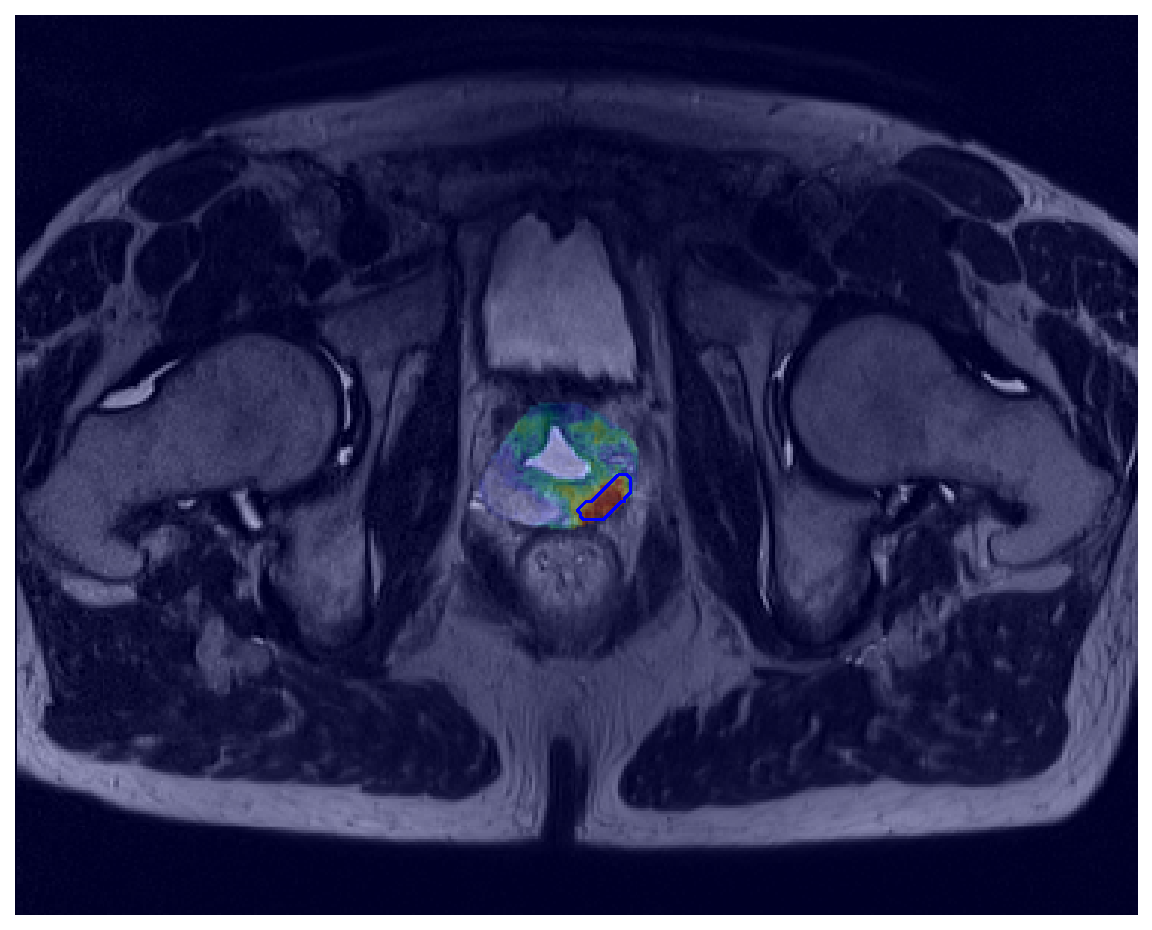
\includegraphics[width=.45\textwidth]{6_pipeline/figures/examples/patient_634.pdf}}
  \hfill
  \subfigure[\acs*{auc} = 0.942]{\label{fig:pat778}\includegraphics[width=.45\textwidth]{6_pipeline/figures/examples/patient_778.pdf}}
  \hfill
  \subfigure[\acs*{auc} = 0.914]{\label{fig:pat1036}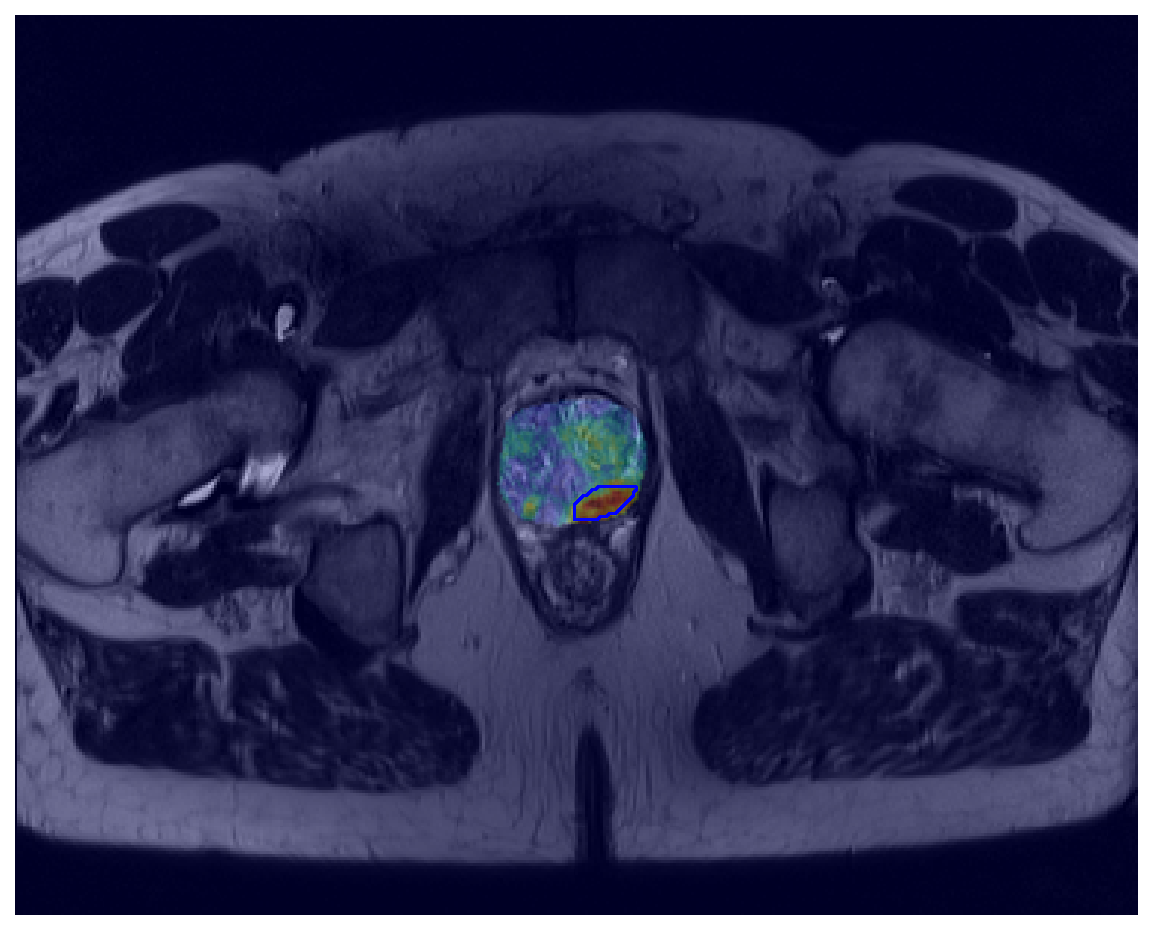
\includegraphics[width=.45\textwidth]{6_pipeline/figures/examples/patient_1036.pdf}}
  \hspace*{\fill}\\
  \hspace*{\fill}
  \subfigure[\acs*{auc} = 0.692]{\label{fig:pat634}\includegraphics[width=.45\textwidth]{6_pipeline/figures/examples/patient_410.pdf}}
  \hfill
  \subfigure[\acs*{auc} = 0.879]{\label{fig:pat778}\includegraphics[width=.45\textwidth]{6_pipeline/figures/examples/patient_784.pdf}}
  \hfill
  \subfigure[\acs*{auc} = 0.735]{\label{fig:pat1036}\includegraphics[width=.45\textwidth]{6_pipeline/figures/examples/patient_1041.pdf}}
  \hspace*{\fill}
  \caption[Illustration the resulting detection of our \acs*{mpmri} \acs*{cad} for \acs*{cap} detection.]{Illustration the resulting detection of our \acs*{mpmri} \acs*{cad} for \acs*{cap} detection. The blue contours corresponds to the \ac{cap} while the \texttt{jet} overlay represents the probability.}
  \label{fig:resultcad}
\end{figure}
\end{landscape}

As previously done, the experiment is performed in a \ac{lopo} fashion and a \ac{roc} analysis is carried out.
The comparative results are shown in \acs{fig}\,\ref{fig:res-Ex4}.
In overall, classification using the fine-tuned features improve the classification performance.
The third classification configuration is, however, the one which outperforms others with an \ac{auc} of $0.836 \pm 0.083$.
The improvement in terms of \ac{auc} is of $0.028$ and $0.050$ compared with the 1\textsuperscript{st} and 2\textsuperscript{nd}, respectively.

In clinical setting, the \ac{auc} score is categorized in 3 levels: (i) ``acceptable'' discrimination for an \ac{auc} ranging from $0.7$ to $0.8$, (ii) ``excellent'' discrimination for an \ac{auc} ranging from $0.8$ to $0.9$, and ``outstanding'' discrimination when the \ac{auc} is over $0.9$~\cite{hosmer2004applied}.
Therefore, the combination of all \ac{mri} modalities in conjunction with fine-tuning allow to upgrade our \ac{cad} system from an ``acceptable'' to an ``excellent'' discrimination level.

Additionally, the individual \ac{roc} analysis for each patient for the best configuration is shown in \acs{fig}\,\ref{fig:indauc}.
It can be noted that 12 patients have an \ac{auc} superior to $0.800$ and 2 patients have a rather low \ac{auc} below $0.700$.
Regarding the 4 patients with an \ac{auc} below $0.800$, 3 patients have a \ac{cap} localized in the \ac{cg}.

To illustrate qualitatively the results of our \ac{mpmri} \ac{cad} system, 6 diverse examples are presented in \acs{fig}\,\ref{fig:resultcad} by overlapping the probability map of having a \ac{cap} with the original \ac{t2w}-\ac{mri} slice.

\subsection{Benefit of the \acs*{mrsi} modality}\label{subsec:chp6:exp-res:Ex5}

\begin{figure}
  \centering
  \includegraphics[width=0.7\linewidth]{6_pipeline/figures/exp-6/stacking_wt_mrsi.pdf}
  \caption{Illustration of the gain of including the \acs*{mrsi} modality in a \acs*{mpmri} \acs*{cad}.}
  \label{fig:resmrsigain}
\end{figure}

We recall that the goal of this thesis is to use all the \ac{mpmri} modalities.
In this regard, \ac{mrsi} has nearly never been used together with the other modalities --- i.e., \ac{t2w}-\ac{mri}, \ac{dce}-\ac{mri}, and \ac{adc} map --- apart of the recent work of \citeauthor{trigui2017automatic}~\cite{trigui2016classification,trigui2017automatic}.
Therefore, we propose in this experiment to compare the classification performance by removing the \ac{mrsi} features.
In this regard, we propose to train 2 stacking classifiers --- with a \ac{gb} as meta-classifier --- while removing the feature related to \ac{mrsi} for one of them.
The same \ac{lopo} validation model is used as before and the results obtained from \ac{roc} analysis are depicted in \acs{fig}\,\ref{fig:resmrsigain}.

Therefore, including \ac{mrsi} into the classification pipeline increases the \ac{auc} from $0.756 \pm 0.092$ to $0.786 \pm 0.098$ for a gain of $0.030$.

\section{Methodology}\label{sec:chp6:method}

\subsection{Materials}

The \ac{mpmri} data are acquired from a cohort of patients with
higher-than-normal level of \ac{psa}.
Acquisition is achieved with a \SI{3}{\tesla} whole body
\ac{mri} scanner (Siemens Magnetom Trio TIM, Erlangen, Germany) using
sequences to obtain \ac{t2w}-\ac{mri}, \ac{dce}-\ac{mri},
\ac{dw}-\ac{mri}, and \ac{mrsi}.
In addition of the \ac{mri} examination, these patients also have undergone
a \ac{trus} guided-biopsy.
The dataset is composed of a total of 19 patients, 17 of which
have biopsies that were positive for \ac{cap} and 2 patients are considered
``healthy'' because they have negative biopsies.
In all 12 patients have a \ac{cap} in the \ac{pz}, 3 patients
have \ac{cap} in the \ac{cg}, 2 patients have invasive \ac{cap} in
both the \ac{pz} and the \ac{cg}, and 2 patients are considered
``healthy''.
An experienced radiologist segmented the prostate organ --- on
\ac{t2w}-\ac{mri}, \ac{dce}-\ac{mri}, and \ac{adc} --- as
well as the prostate zones --- i.e., \ac{pz} and \ac{cg} ---, and
\ac{cap} on the \ac{t2w}-\ac{mri}.
The full description and the data set are available at \acs*{iccvb}
website\footnote{\url{http://i2cvb.github.io/}}~\cite{Lemaitre2016thesis}.

\subsection{\acs*{cad} pipeline for \acs*{cap}}

Our \ac{mpmri} \ac{cad} system consists of 7 different steps:
pre-processing, segmentation, registration, feature detection, feature
balancing, feature selection/extraction, and finally classification.
%% It should be noted that \ac{cad} system designed deals with
%% multiparametric \ac{mri} data.

\subsubsection{Pre-processing}\label{subsec:chp6:method:PP}

Normalization is, a crucial step to reduce the inter-patient
variations which allows to improve the learning during the
classification stage.
However, the \ac{mri} modalities provide specific type of data --- static
\emph{vs.} dynamic information, images \emph{vs.} signals --- that
required a dedicated pre-processing.
Therefore, we pre-process differently the data:
\ac{t2w}-\ac{mri} is normalized using a Rician
a-priori that has been shown to be better than the traditional
$z$-score~\cite{lemaitre2016normalization}.
In contrast to \ac{t2w}-\ac{mri}, in \ac{adc} map the \ac{pdf} within the
prostate does not follow a known distribution and thus one cannot use
a parametric model to normalize these images and a non-parametric
piecewise-linear normalization~\cite{Nyul2000} is the best option for
this case.
\ac{dce}-\ac{mri} is a dynamic sequence and the data are normalized
based on a mean kinetic expression registration as proposed
in~\cite{Lemaitre2016thesis}.
Finally, the \ac{mrsi} modality has been pre-processed to correct the
phase, suppress the baseline, and align the frequencies~\cite{Parfait2012}.

\subsubsection{Segmentation and registration}\label{subsec:chp6:method:Seg-Reg}

For this work, our radiologist has manually segmented the prostate
organs on the different modalities.
However, the segmented prostate needs to be registered before to
extract features.
The \ac{t2w}-\ac{mri} is used as reference and each segmented prostate
in other modalities are registered to this reference.
Indeed, three registrations are used to correct: (i) the patient
motion during the \ac{dce}-\ac{mri} acquisition, (ii) the patient
motion between the \ac{t2w}-\ac{mri} and the \ac{dce}-\ac{mri}
acquisitions, and (iii) the patient motion between the
\ac{t2w}-\ac{mri} and the \ac{adc} map acquisition.
Additionally, volumes from all modalities have been interpolated to the
resolution of \ac{t2w}-\ac{mri}.

\subsubsection{Feature detection}\label{subsec:chp6:method:fea-det}
Similarly to the pre-processing, specific features are extracted
depending of the specificity of each \ac{mri} modality.
\begin{description}[style=unboxed,leftmargin=0cm]
\item[\ac{t2w}-\ac{mri} and \ac{adc} map features]
Additionally to the normalized intensity, edge- and texture-based
features are commonly extracted from \ac{t2w}-\ac{mri} and \ac{adc}
map.
The following set of filters characterizing edges have been used: (i)
Kirsch, (ii) Laplacian, (iii) Prewitt, (iv) Scharr, (v) Sobel, and
(vi) Gabor.
Except for the Kirsch filter, the other filters are applied in 3D,
taking advantage of the volume information instead of slice
information, as it is usually done.
Additionally, features based on phase congruency are
computed~\cite{kovesi1999image}.
To characterize the local texture, both second-order \ac{glcm}-based
features~\cite{Haralick1973} and rotation invariant and uniform
\ac{lbp}~\cite{ojala2002multiresolution} are extracted.
To encode 3D information, the 13 first Haralick features are computed
for the 13 possible directions.
For the same reason, the \ac{lbp} codes are computed for the
three-orthogonal-planes of each \ac{mri} volume.
All these features are extracted at each voxel of the volume.

\item[\ac{dce}-\ac{mri} features]
In brief, the entire enhanced signal, semi-quantitative~\cite{Huisman2001}, and
quantitative-based
models~\cite{brix1991pharmacokinetic,hoffmann1995pharmacokinetic,tofts1995quantitative,giannini2015fully}
are computed.

\item[\ac{mrsi} features]
Three different techniques are used to extract
discriminative features: (i) relative quantification based on
metabolite quantification, (ii) relative
quantification based on bounds integration, and (iii) spectra
extraction from \SIrange{2}{4}{\ppm}~\cite{Lemaitre2016thesis}.

\item[Anatomical features]
Four different metrics are computed based on the relative distance to the
prostate boundary as well as the prostate center, and the relative
position in the Euclidean and cylindrical coordinate
systems~\cite{Chen2002,Litjens2014}.

\end{description}

\subsubsection{Feature balancing}\label{subsec:chp6:method:fea-bal}
Imbalanced dataset is a common problem in medical imaging.
The number of cancerous voxels is much lower than the number of
``healthy'' voxels for a patient.
However, the problem of imbalanced dataset compromises the learning
process.
solving the problem of imbalanced is equivalent to under- or
over-sampling part of the dataset to obtain equal number of samples
in both classes.
We used several methods and selected the most efficient for our
dataset~\cite{imblearn}.

\subsubsection{Feature selection and extraction}\label{subsec:chp6:method:fea-sel}

Feature selection and extraction are used in our experiment.
\ac{mrsi} and \ac{dce}-\ac{mri} are decomposed using three feature
extraction methods: \ac{pca}, sparse-\ac{pca}, and \ac{ica} are used
to decompose signal-based data.
Additionally to feature extraction, two methods of feature selection
are used: (i) the one-way \ac{anova} and (ii) the Gini importance
obtained while learning the \ac{rf} classifiers.

\subsubsection{Classification}\label{subsec:chp6:method:clas}

\ac{rf} has been chosen as our base classifier --- allowing for
feature selection as well --- to perform classification of individual
modality as well as the combination of modalities.
Additionally, we use stacking to create ensemble of base learners
using a meta-classifier~\cite{wolpert1992stacked}, namely \ac{adb} and \ac{gb}.

\section{Results and evaluation} \label{sc:results}
\begin{figure}
\centering
 \includegraphics[width=0.9\linewidth]{Figures/combine_all.pdf}
  \caption[Analysis of feature combination approaches after fine
  tuning.]{Analysis of feature combination approaches after fine
    tuning through balancing and feature selection/extraction.}
  \label{fig:res-Ex4}
\end{figure}

%\begin{figure}
%  \centering
%  \includegraphics[width=0.7\linewidth]{Figures/plot_all_patients.pdf}
%  \caption{Individual patient \acs*{auc} for the best configuration
%  of the \acs*{mpmri} \acs*{cad}.}
%  \label{fig:indauc}
%\end{figure}
Various experiments were run in order to optimize the balancing and
the feature selection strategies~\cite{Lemaitre2016thesis}.
We found that once all features are concatenated together,
\ac{nm3}~\cite{mani2003knn} is the method providing the best
enhancement of the classification performance with an \ac{auc} of $0.824 \pm
0.076$.
Therefore, with this optimal balancing, were here report the
final step consisting of three strategies:
(i) the selected features from each modality (i.e., 331 features) are
concatenated together and used in a \ac{rf} classifier,
(ii) the selected features from each modality (i.e., 331 features) are
used to train a stacking classifier with a \ac{gb} as meta-classifier, and
(iii) the selected features from the concatenated set of feature
(i.e., 267 features) are used to train a single \ac{rf} classifier.

%\begin{landscape}
\begin{figure}
  \hspace*{\fill}
  \subfigure[\acs*{auc} =
  0.922]{\label{fig:pat634}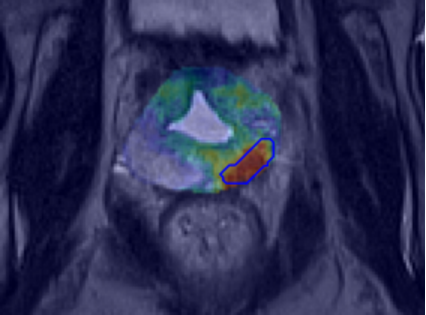
\includegraphics[width=.45\linewidth]{Figures/patient_634_foc.pdf}}
 \hfill
  %\subfigure[\acs*{auc} =
  %0.942]{\label{fig:pat778}\includegraphics[width=.20\textwidth]{Figures/patient_778.pdf}}
  %\hfill
 \subfigure[\acs*{auc} =
 0.914]{\label{fig:pat1036}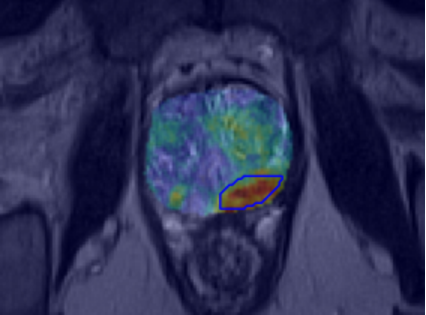
\includegraphics[width=.45\linewidth]{Figures/patient_1036_foc.pdf}}
 \hspace*{\fill}
 % \hspace*{\fill}
%  \subfigure[\acs*{auc} = 0.692]{\label{fig:pat634}\includegraphics[width=.45\textwidth]{Figures/patient_410.pdf}}
 % \hfill
 % \subfigure[\acs*{auc} = 0.879]{\label{fig:pat778}\includegraphics[width=.45\textwidth]{Figures/patient_784.pdf}}
 % \hfill
 % \subfigure[\acs*{auc} = 0.735]{\label{fig:pat1036}\includegraphics[width=.45\textwidth]{Figures/patient_1041.pdf}}
 % \hspace*{\fill}
  \caption[Illustration the resulting detection of our \acs*{mpmri}
  \acs*{cad} for \acs*{cap} detection.]{Illustration the resulting
    detection of our \acs*{mpmri} \acs*{cad} for \acs*{cap}
    detection. The blue contours corresponds to the \ac{cap} while the
    jet overlay represents the probability.}
  \label{fig:resultcad}
\end{figure}
%\end{landscape}

The experiments were performed in a \ac{lopo} fashion and a \ac{roc}
analysis is carried out.
The comparative results are shown in \acs{fig}\,\ref{fig:res-Ex4}.
In overall, classification using the fine-tuned features improve the
classification performance.
The third classification configuration is, however, the one which
outperforms others with an \ac{auc} of $0.836 \pm 0.083$.
The improvement in terms of \ac{auc} is of $0.028$ and $0.050$
compared with the 1\textsuperscript{st} and 2\textsuperscript{nd}
configurations, respectively.

In clinical setting, the \ac{auc} score is categorized in 3 levels:
(i) ``acceptable'' discrimination for an \ac{auc} ranging from $0.7$
to $0.8$, (ii) ``excellent'' discrimination for an \ac{auc} ranging
from $0.8$ to $0.9$, and ``outstanding'' discrimination when the
\ac{auc} is over $0.9$~\cite{hosmer2004applied}.
Therefore, the combination of all \ac{mri} modalities in conjunction
with fine-tuning allow to upgrade our \ac{cad} system from an
``acceptable'' to an ``excellent'' discrimination level.

To illustrate qualitatively the results of our \ac{mpmri} \ac{cad}
system, 2 diverse examples are presented in
\acs{fig}\,\ref{fig:resultcad} by overlapping the probability map of
having a \ac{cap} with the original \ac{t2w}-\ac{mri} slice.

\section{Conclusion}

In this paper, we presented one of the the first \ac{cad} system using all
the \ac{mpmri} modalities for prostate cancer detection.
Indeed, \ac{mrsi} has nearly never been used together with the other
modalities.
With an extensive validation approach to select the best
features, the best balancing strategy as well as the best classifier,
we obtained results on a rather complicated dataset of 17 patients
with an average \ac{auc} of $0.836 \pm 0.083$ which put our system in the
state-of-the-art, even so different \ac{cad}s were tested on different
datasets.

% \section{Conclusion} \label{sc:final-remarks}

The latest denoising techniques have been compared to the more conventional ones on a set of synthetic images onto which various noise types have been added as well as on \ac{sdoct} images.
In general \ac{bm3d}, \ac{pgpd}, and K-SVD led to the best results and should be regarded as the main techniques for denoising \ac{sdoct} images which inherently have speckle noise.
Future work will focus on recent techniques, BM4D~\cite{Maggioni} which benefits from the data structure (volume) of the \ac{sdoct} images as well as the recent work of Sheet~\emph{et~al.}~\cite{7163987} using deep learning to tackle the segmentation and the denoising in once.
Another interesting work will be to fully investigate, through classification performance, the effect of the selected noise removal techniques on a full pipeline of \ac{sdoct} volume for \ac{dme} classification~\cite{lemaitre2015classification}.
% \section{Acknowledgments}
The authors would like to thank the VIBOT and MsCV students from the University of Burgundy for their involvement in this paper. The authors would also like to thank the Regional Council of ``Bourgogne Franche-Comt\'e'' for partially funding this work.

% Bibliography
\bibliographystyle{IEEEtran}
%\IEEEtriggeratref{10}
\bibliography{Bibliography}

\end{document}
